\chapter{Results}
\label{ch:results}

\emph{In this chapter the results of the experiments and methods detailed in Chapters \S\ref{ch:background} and \S\ref{ch:methodology} are presented.}
\emph{A detailed analysis of the results is included along with references to similar results within the literature.}
\emph{Both quantitative and qualitative analysis is carried out and the limitations of the metrics used are discussed.}

\emph{First, the reproduction of {\scshape Steering Clear} \citep{steering-clear} detailed in \cref{sec:steering-clear} is presented.}
\emph{Comparisons to the original paper are made along with additional analysis.}

\emph{Finally, the natural language setting described in \cref{sec:prompt-pairs} is analysed.}
\emph{A comparison to the {\scshape Steering Clear} toy environment is made.}
\emph{The suitability of the quantitative metrics proposed in \cref{sec:prompt-pairs} is discussed.}

\section{{\scshape Steering Clear} Reproduction}
\label{sec:steering-clear-res}

The results of the reproduction suggest that the analysis by \citet{steering-clear} are sound though an exact replication was not achieved.

\begin{figure}
    \centering
    \captionsetup{width=.9\textwidth}
    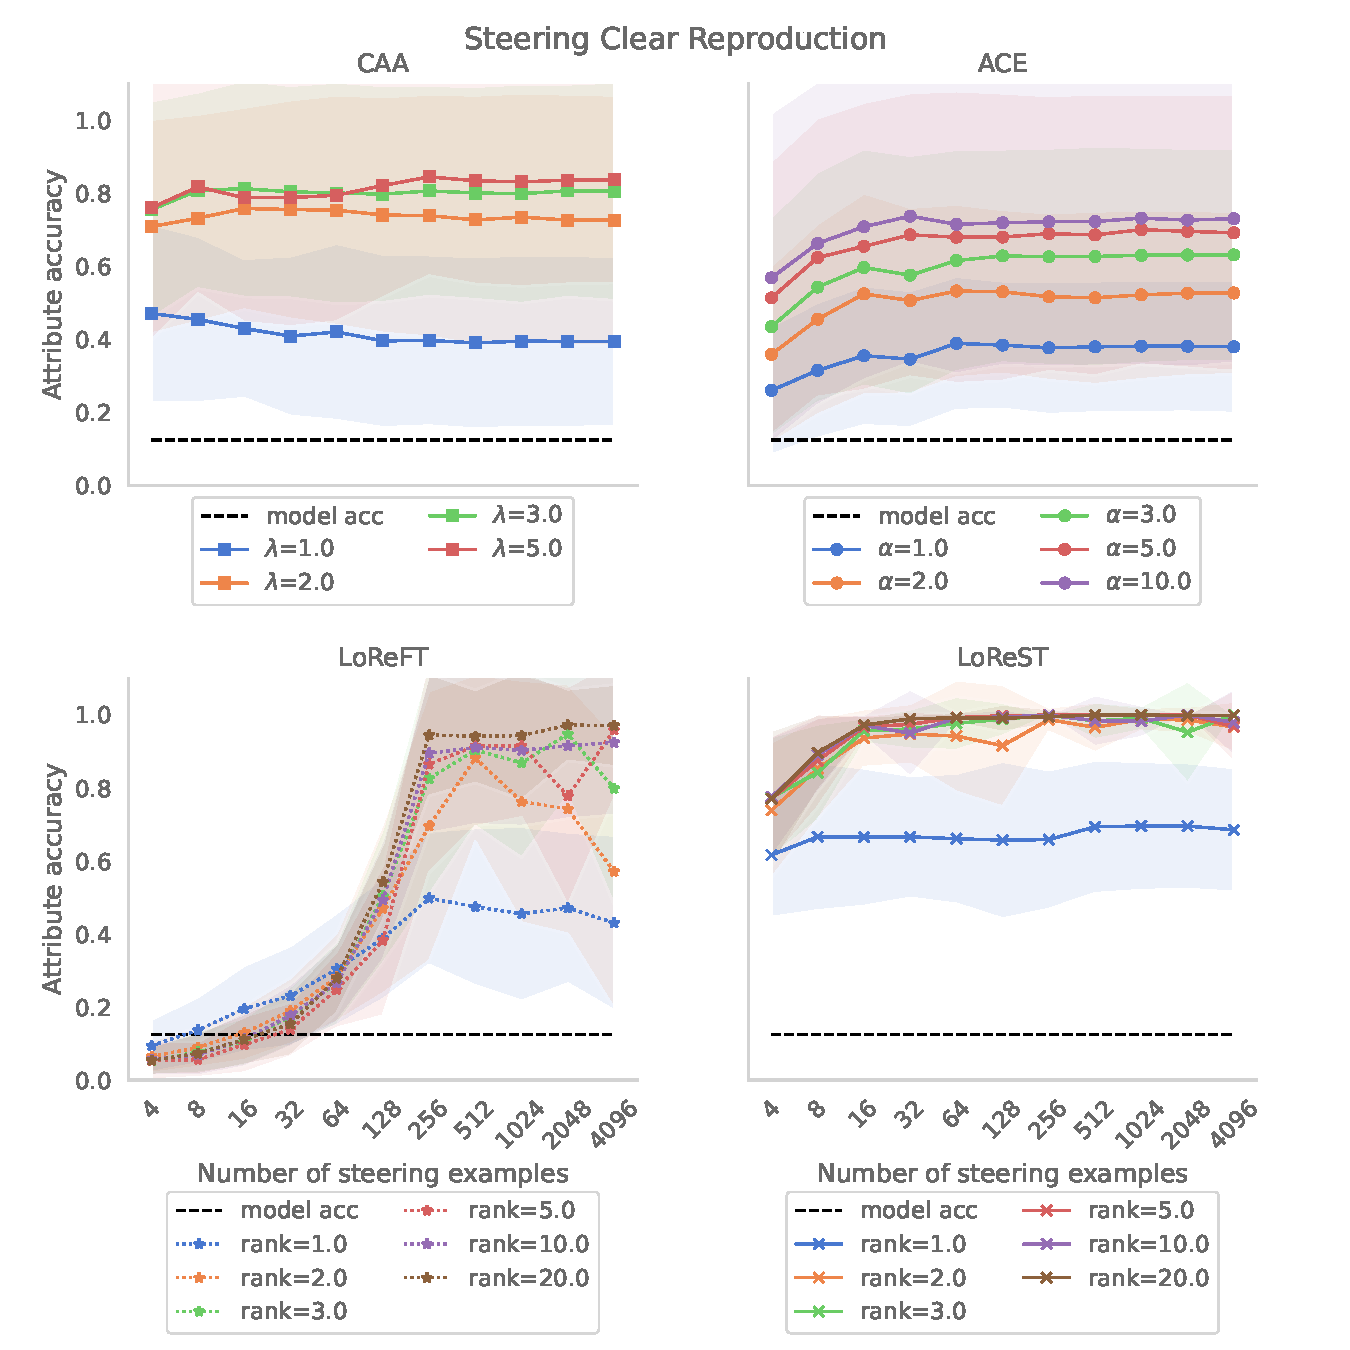
\includegraphics[width=\textwidth]{figures/steering_clear.pdf}
    \caption{
        The average accuracy of the steered model predicting the correct attribute value, in all cases this is $\mu_1$ (see \cref{sec:steering-clear}).
        This represents how well the adaptor was able to steer the models output towards the correct value for the given attribute.
        In contrast to Figure 1 in \citet{steering-clear} only the target attribute is considered in comparison to all attributes.
        The same trends of consistent performance for affine methods and a clear increase in performance for low-rank methods are present as in \citet{steering-clear}.
    }
    \label{fig:steering-clear}
\end{figure}

The results of \cite{steering-clear} are reproduced in \cref{fig:steering-clear} following the experimental setup in \cref{sec:steering-clear}.
There are a few changes from Figure 1 in \cite{steering-clear}, primarily the steering metric focuses on the steered attribute rather than entire output label.
Furthermore, ACE is added and minimally modified counterfactuals (MiMiC) \citep{mimic} is removed.
A full discussion of the different metric and why this was used is presented in \cref{app:steering-clear}.

The figure clearly shows a difference between the linear/affine methods of CAA \& ACE and the low-rank methods of LoReFT \& LoReST.
In the limit of more examples both low-rank methods achieve near 100\% success rate in steering the target attribute to the target value.
In comparison the affine methods reach an asymptote (${\footnotesize \sim} 0.8$ for most hyperparameters) which does not increase with more training examples.
Importantly, in the low training example setting LoReFT performs worse than both CAA and ACE.
In fact, it performs worse than the model without steering.
This is due to the requirement to train parameters which both affine approaches lack.
However, the addition of parameters allows the method to perform better as more examples are presented.
This feature of improvement with more examples is shared with LoReST.

Across the methods there is a critical hyperparameter value above which the adaptors performance does not significantly improve.
In the case of CAA this appears to be $\lambda=2$; for LoReFT the threshold rank is likely 3 as 2 decreases in accuracy as more examples are introduced; finally with LoReST the rank is clearly 2.
ACE behaves differently due to it's design (detailed in \cref{sec:ace}) where the parameters relate to the strength of the behaviour more directly.
This is visible in \cref{fig:steering-clear} as clear bands as the hyperparameter increases; in comparison to the other plots where after a threshold hyperparameter value the adaptors behave similarly.

Similar to the findings of \citet{steering-clear} LoReFT plateaus after 256 examples which coincides with the dimension of the activation space.
This distinction is not present in the other methods though this is similar to the Figure in \citet{steering-clear}.
A possible explanation for this in the case of the affine methods is they do not learn their own representation.
Instead, with sufficient opposing examples, the difference in steering direction is minimal with more examples.

LoReST in comparison to both LoReFT and the affine methods incorporates both affine steering and low-rank steering.
This means in the low data regime it behaves closer to ACE and CAA relying on the bias term; when enough data is provided LoReST can encode the concepts sufficiently resulting in an increase in accuracy.
This is supported by the fact that LoReST achieves an accuracy of ${\footnotesize \sim} 0.8$ with 4 examples matching CAA, and then LoReST then continues to increase in accuracy eventually plateauing at the same accuracy as LoReFT, ${\footnotesize \sim} 1.0$.
This behaviour matches those presented in \citet{steering-clear}.

\subsection{The Issue of Variance}

The variance of the adaptors was not considered in \citet{steering-clear} even though, as \cref{fig:steering-clear} demonstrates, this can be quite high.
The variance that is presented in \cref{fig:steering-clear} is the standard deviation (std) across the 20 runs, this has been clipped to fit in the range 0-1.\footnote{This problem is due to the skewed success distribution.}
\citet{steerability} demonstrate that, when considering the std of the adaptors, many datasets that appear steerable have a significant chance of failing.

It is very important to consider the variance as the use case of steering vectors requires a high rate of success.
This is especially the case when the variability includes steering in the \emph{opposite} direction.

As \cref{fig:steering-clear} demonstrates the affine methods have the highest std.
This is expected as these methods rely primarily on the means of the sampled steering examples which can vary a lot especially in the low data regime.

In the case of CAA the mean std is $0.28$, this means that for $\lambda \in [3..5]$ the adaptor performs anywhere from as low as $0.5$ accuracy up to $1.0$ accuracy.
Similarly, ACE has a mean std of $0.30$ which has a similar effect as CAA.

This is in contrast to the low rank approaches which have a tighter std especially LoReST.
In the case of LoReFT the mean std is $0.15$ half that of the affine methods.
Furthermore, this increases with the number of examples with only 4 examples the mean std is $0.05$ whereas for 4096 the mean std is $0.26$.

LoReST has the best variance with a mean std of $0.08$.
Ignoring $rank=1$, which has the worst variance, results in a mean std of $0.06$ which decreases substantially after 16 examples down to a mean std of $0.04$.

All together this suggests that LoReST is the ideal adaptor as it has a large success range regarding the number of provided examples whilst exhibiting very low variance in success.
As is demonstrated in the next section LoReST continues to have the lowest variance but does not fair well on LLMs.

\section{Prompt Pairs}
\label{sec:prompt-pairs-res}

\subsection{Quantitative Analysis}
\label{sec:quant}

Recall the three metrics defined in \cref{sec:prompt-pairs} of target SAE feature activation proportion, spurious SAE feature activation proportion and semantic similarity.
As there is no notion of accuracy akin to \citet{steering-clear} the closest comparison comes from the activation of SAE features.
To avoid indiscriminate increase across all SAE features, the spurious SAE features verifies the model only affects the target concepts.

The two SAE metrics are presented together for each adaptor.
This presents a full picture of how discriminating the model is towards the desired concept.
The target behaviour would be for high target SAE proportion, close to 1, and low spurious SAE proportion, close to 0.
This would suggest the adaptor successfully steers the model towards the target concepts without effecting the features that are not related to the context.

\subsubsection{CAA}

\begin{figure}
    \centering
    \captionsetup{width=.9\textwidth}
    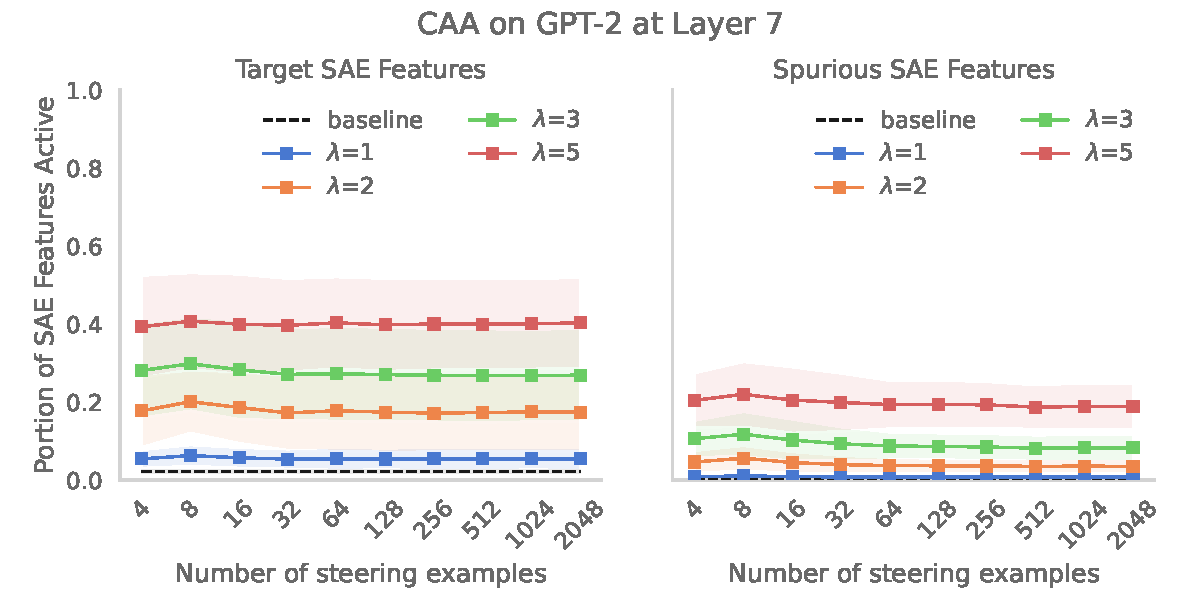
\includegraphics[width=\textwidth]{figures/gpt2_7_caa.pdf}
    \caption{
        The proportion of target SAE features that were activated by CAA as a function of the number of steering examples, alongside the proportion of spurious SAE features that were activated by CAA.
        Higher target SAE proportion and lower spurious SAE proportion is better.
    }
    \label{fig:gpt-caa}
\end{figure}

\cref{fig:gpt-caa} presents the two SAE metrics for CAA good performance.
This closely matches the behaviour that was seen in \citet{steering-clear} with the higher ranks performing better.

The inclusion of the spurious feature metric demonstrates a key tradeoff when steering models.
The stronger the intervention the more the target representation is present but the more spurious representations are also present.
Compare $\lambda = 5$, which has a target feature proportion of $0.40 \pm 0.11$ and spurious proportion of $0.19 \pm 0.07$, with $\lambda = 1$, which has a target proportion of $0.06 \pm 0.03$ and spurious of $0.01 \pm 0.00$.

Though CAA does not achieve a target proportion above $0.5$ recall the definition of the metric in \cref{sec:prompt-pairs}.
The average SAE activation vector is far less sparse than a single activation vector, therefore the output SAE vector is likely to only activate a small fraction of the average SAE activations.

As with \citet{steering-clear} the metric remains consistent across the number of steering examples.
Take $\lambda = 5$ the standard deviation in the mean is only $0.00002$ for the target features and $0.0001$ for the spurious features.

\subsubsection{ACE}

\begin{figure}
    \centering
    \captionsetup{width=.9\textwidth}
    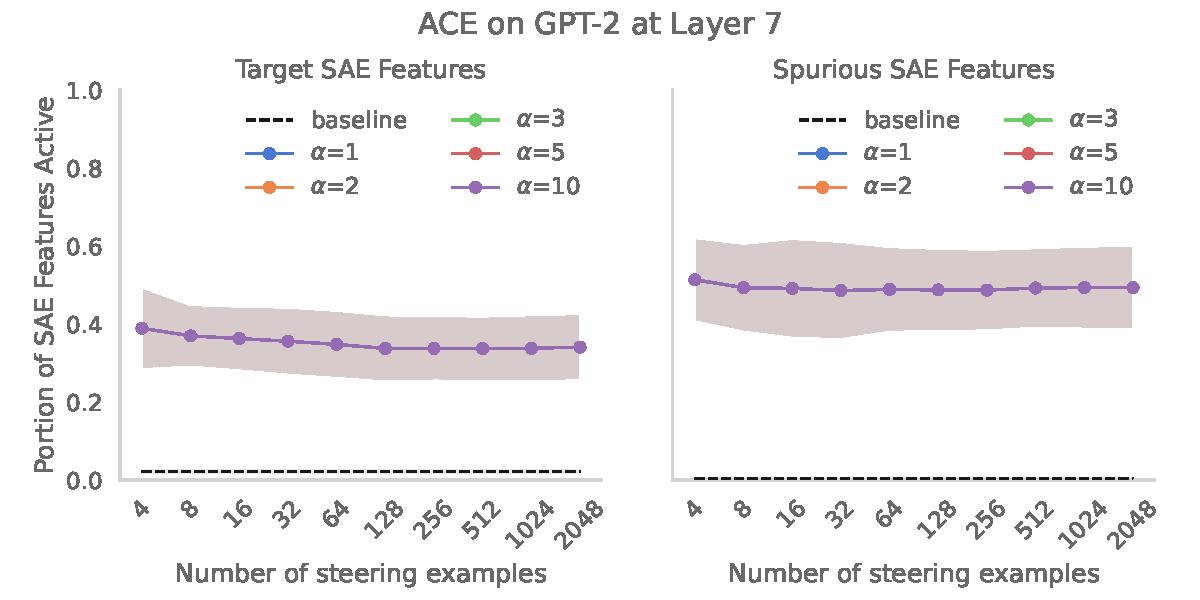
\includegraphics[width=\textwidth]{figures/gpt2_7_ace.pdf}
    \caption{
        The proportion of target SAE features that were activated by ACE as a function of the number of steering examples, alongside the proportion of spurious SAE features that were activated by ACE.
        Higher target SAE proportion and lower spurious SAE proportion is better.
    }
    \label{fig:gpt-ace}
\end{figure}

The two SAE metrics for ACE are presented in cref{fig:gpt-ace}.
Unlike in \citet{ace} and the results in \cref{fig:steering-clear} ACE appears to perform very badly.
It is able to achieve a promising target feature proportion of $0.35$ however this is accompanied by a spurious feature proportion of $0.49$.
This means that ACE is introducing more spurious features than it is aligning towards target features.

The reason for this is unclear as \citet{ace} show promising results for the adaptor and \cref{fig:steering-clear} suggests the method can work.
The issue is likely with the model used, GPT-2, rather than the one used in \citet{ace}, Llama 3 \citep{llama3}.
GPT-2, though able to produce fairly coherent English sentences does not have the reasoning capabilities of larger models such as Llama 3.
For this reason the internal representations likely do not have a meaningful baseline for ACE to utilise.

\subsubsection{LoReFT}

\begin{figure}
    \centering
    \captionsetup{width=.9\textwidth}
    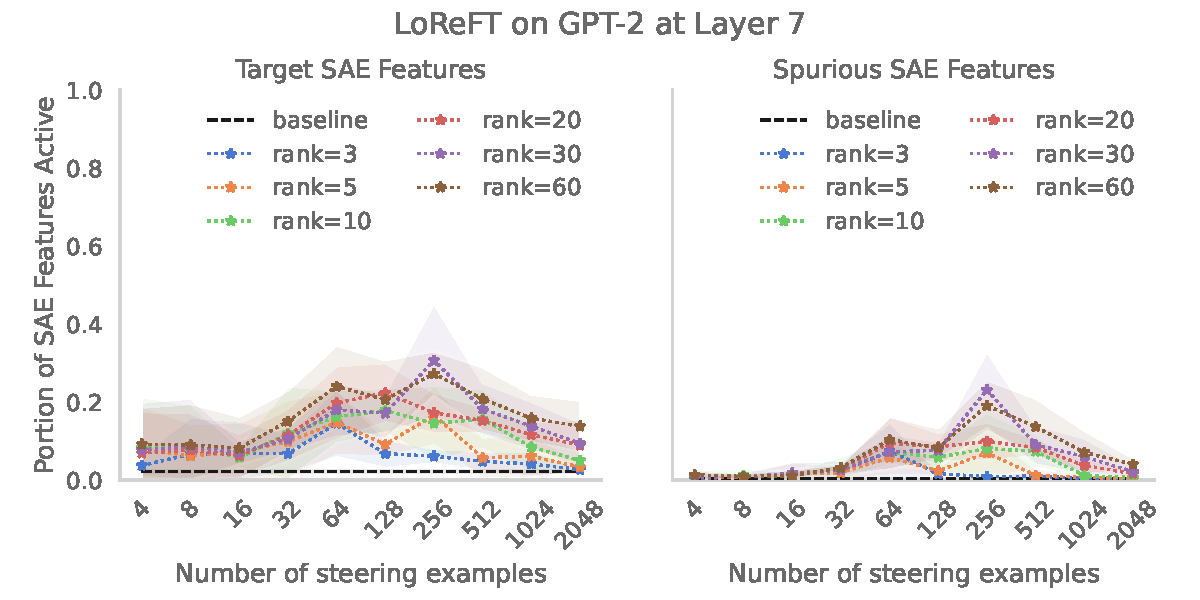
\includegraphics[width=\textwidth]{figures/gpt2_7_loreft.pdf}
    \caption{
        The proportion of target SAE features that were activated by LoReFT as a function of the number of steering examples, alongside the proportion of spurious SAE features that were activated by LoReFT.
        Higher target SAE proportion and lower spurious SAE proportion is better.
    }
    \label{fig:gpt-loreft}
\end{figure}

In comparison to the \textsc{Steering Clear} environment the low rank methods appear to perform worse in regards to the SAE metrics.
The results for LoReFT are presented in \cref{fig:gpt-loreft} and demonstrate a lower target feature activation in comparison to both affine approaches.

The best performing rank is $rank = 30$ with 256 examples which achieves $0.31 \pm 0.15$ target feature proportion in comparison to CAA which achieves $0.40 \pm 0.11$.
The spurious feature proportion for $rank = 30$ is $0.23 \pm 0.10$ also higher than CAA with $0.19 \pm 0.07$.

The potential benefit of LoReFT occurs at the larger values where the spurious feature proportion drops but the target proportion remains relatively high.
For example, with $rank = 60$ the target proportion is $0.14 \pm 0.06$ and the spurious proportion is $0.04 \pm 0.02$.
Compare this to CAA where $\lambda = 5$ has a better target proportion, $0.40 \pm 0.11$, but a worse spurious proportion, $0.19 \pm 0.06$.
This does come at the cost of having to tune hyperparameters for LoReFT.

It is possible with a higher rank LoReFT may perform much better.
Given the trends seen in \cref{fig:steering-clear} it is unlikely more examples will help as after 256 examples the approach plateaus.

\subsubsection{LoReST}

\begin{figure}
    \centering
    \captionsetup{width=.9\textwidth}
    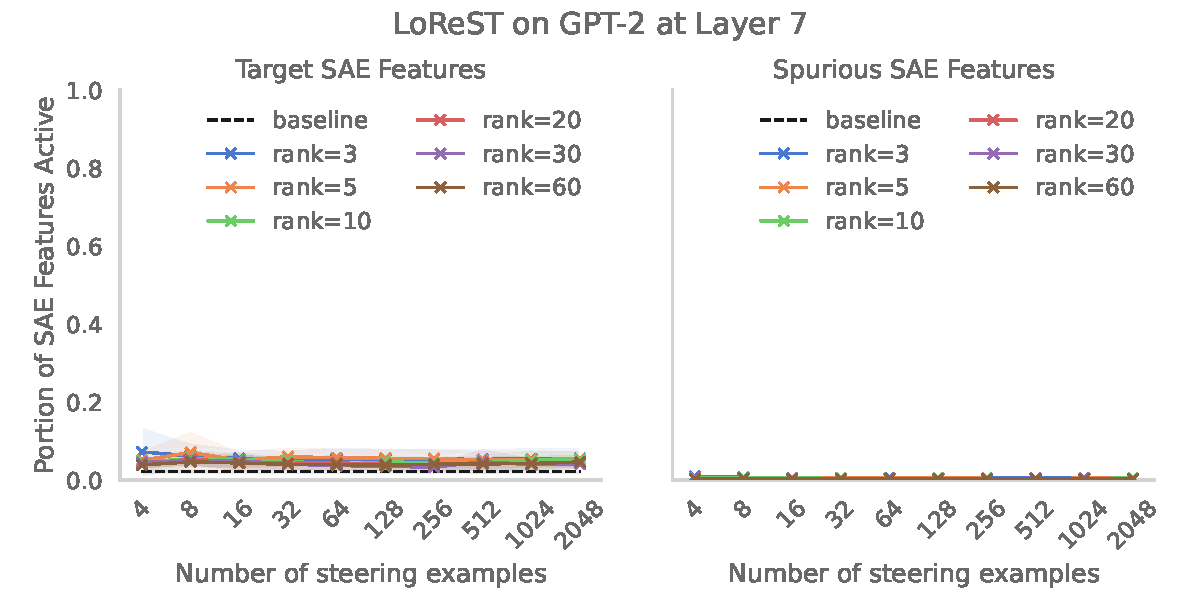
\includegraphics[width=\textwidth]{figures/gpt2_7_lorest.pdf}
    \caption{
        The proportion of target SAE features that were activated by LoReST as a function of the number of steering examples, alongside the proportion of spurious SAE features that were activated by LoReST.
        Higher target SAE proportion and lower spurious SAE proportion is better.
    }
    \label{fig:gpt-lorest}
\end{figure}

\cref{fig:gpt-lorest} presents the two SAE metrics achieved by LoReST.
Compared to the previous 3 approaches this suggests very poor performance from LoReST.
All ranks appear to perform at the same level reaching only $0.05 \pm 0.00$ on average across all hyperparameters.
This is marginally above the baseline value of $0.02 \pm 0.00$.

The key takeaway however is how well it supresses the spurious features.
In the worst case, $rank = 3$ with 4 examples, LoReST suffers from $0.01 \pm 0.00$ spurious features activated.
Across the full range of hyperparameters the proportion is effectively $0$.

There are a number of possibilities for why the values are so poor.
It may be highly discriminant changing a very small proportion of features that are absolutely necessary hence both the target and spurious SAE proportions are very low.
It may, like LoReFT, require larger ranks or more training examples to properly perform.
It is unlikely due to the model in this case, unlike ACE there is less reliance on meaningful model representations.

\subsubsection{Semantic Similarity}

\begin{figure}
    \centering
    \captionsetup{width=.9\textwidth}
    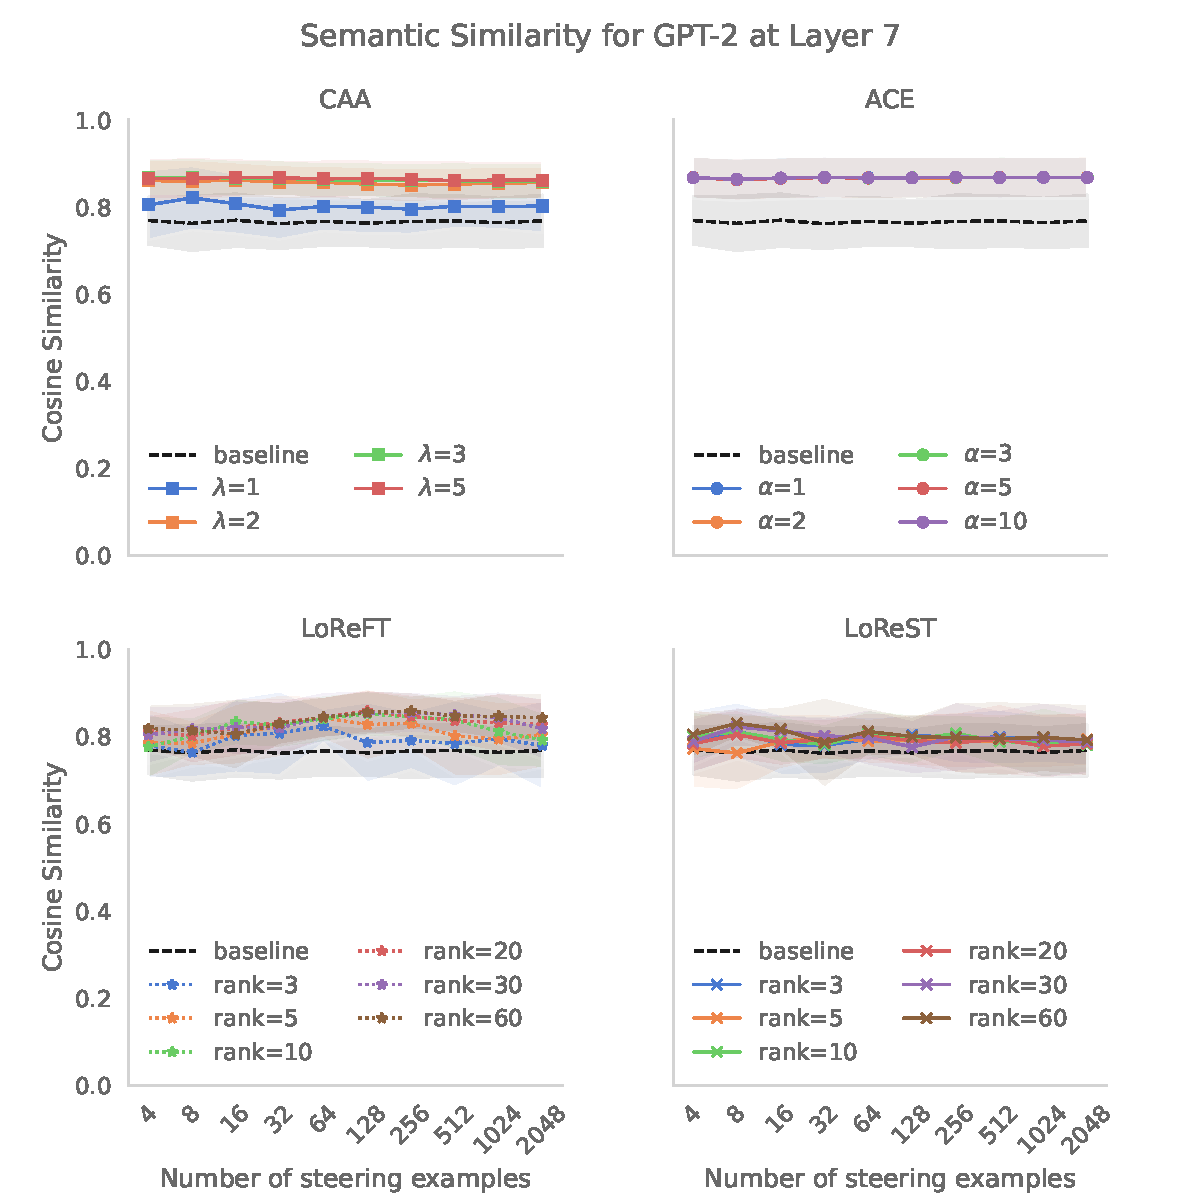
\includegraphics[width=\textwidth]{figures/gpt2_7_similarity.pdf}
    \caption{
        The cosine similarity of Distilbert \citep{distilbert} sentence embeddings for the generated completion.
        The higher the cosine similarity the better the method has performed.
        The number of steering examples is the same as \cref{fig:steering-clear} and the cosine similarity is shared across charts.
    }
    \label{fig:gpt-pp-sim} \end{figure}

The final metric discussed in \cref{sec:prompt-pairs} is semantic similarity which is presented in \cref{fig:gpt-pp-sim}.
As discussed in \cref{sec:prompt-pairs} the semantic similarity is calculated by embedding the target and generated completion using Distilbert \citep{distilbert} and taking the cosine similarity between the two vectors.
A successful adaptor will have a larger semantic similarity with 1 being a perfect match.
The shaded regions in \cref{fig:gpt-pp-sim} represent one standard deviation across the 5 datasets that were used.
The same baseline data is used across all 4 plots.

\smalltitle{CAA} continues to present the same behaviour seen in the previous two metrics.
As the hyperparameter value increases the semantic similarity increases.

The best semantic similarity is achieved by $\lambda = 5$ with $0.86 \pm 0.05$ and in the worst case the adaptor still achieves $0.79 \pm 0.07$ a slight improvement over the baseline at $0.77 \pm 0.06$.
Based on the performance in previous metrics this is the expected result for CAA.

Note that even though $\lambda = 5$ has a larger spurious feature activation in \cref{fig:gpt-caa} it still performs better than the other hyperparameters.
This demonstrates one drawback of this metric on it's own, a high semantic similarity does not mean that the context of the model has been preserved.
This idea is explored further in \cref{sec:qual} where the completions are analysed quantitatively.

\smalltitle{ACE} demonstrates the drawbacks of this metric clearly.
Based on \cref{fig:gpt-ace} the expectation is that ACE would perform poorly.
However, it does produces the highest semantic similarity so it is possible that spurious features do not matter.

The model achieves $0.87 \pm 0.05$, which is not significantly higher than CAA at $0.86 \pm 0.05$, however this performance is consistent across all hyperparameters and example set sizes.

These results may suggest that the effect on spurious correlations are unimportant.
However, as will be shown in \cref{sec:qual} this is not the case and rather the three metrics alone are insufficient to accurately represent the performance of the adaptors.

\smalltitle{LoReFT} performs very erratically though performs better than the baseline on average.
There is no clear relationship between the semantic similarity and the SAE feature activations in \cref{fig:gpt-loreft}.

The best performance is achieved when $rank = 60$ with 256 training examples giving $0.86 \pm 0.04$ on par with CAA and ACE.
This similarity is matched by multiple ranks at this number of examples in particular $rank \in \{10, 20, 30, 60\}$.
In the worst case LoReFT achieves $0.76 \pm 0.08$ comparable to the baseline at $0.77 \pm 0.06$ though slightly worse.

As with the SAE feature activation there is still a large variance in the results.
Given the range of the output the observed variances account for ${\footnotesize \sim} 20\%$ of possible values.

\smalltitle{LoReST} appears to perform the worst on average.
The maximum similarity achieved is $0.83 \pm 0.04$.
The analysis is similar to that of LoReFT with consistent improvement though smaller than the affine methods.
The variance is smaller than that of LoReFT but not significantly so.

Unlike the SAE feature metrics in \cref{fig:gpt-lorest} there appears to be a slight preference towards larger ranks though not significantly so.
Across all steering example sets $rank = 60$ achieves an average similarity score of $0.80$ in comparison to $rank = 3$ which achieves $0.79$.

Overall the three metrics suggest that CAA performs the best across possible training set sizes.
Though it suffers from high variance this is as good, if not better, than the variance of other adaptors.
LoReFT performs comparably but requires tuning hyperparameters and ensuring sufficient training examples are provided.

\subsection{Qualitative Analysis}
\label{sec:qual}

The quantitative metrics analysed in \cref{sec:quant} are useful as a objective comparison across the adaptors, hyperparameters, and number of steering examples.
However, as the environment is based on natural language it is important to analyse the sentences produced as this is the primary output of the LLM.
Along with the analysis in \cref{sec:quant} this will provide a full analysis of the performance of the techniques.

The completions generated by the model with the various adaptors is presented as a \emph{prompt-response} dialogue.
The formatting for these are based on \cites{mwe} dialogues.
For each prompt a range of responses is included across a range of steering examples and hyperparameters.
The same selection of prompts is used across the different tables to provide a consistent comparison across the adaptors.
The specific completions are randomly selected for each adaptor with certain random selections discarded due to their not safe for work nature.

\begin{table}[t!]
    \centering
    \begin{tabular}{c|p{35em}}
        \multicolumn{2}{c}{\textbf{Unsteered model prompt completions}} \\[0.2cm]
        \hline
        examples & \textbf{Disapproval $\to$ Approval} \\
        \hline
        & \dialogue{l}{\prompt{Policy makers often estimate budgets to improve morale and}} \\
        4 & \dialogue{r}{\response{economic growth. But when it comes to national}} \\
        & \dialogue{l}{\prompt{Developers frequently present strategies to reduce misunderstandings and}} \\
        256 & \dialogue{r}{\response{vernacular errors in the future. It is important}} \\
        & \dialogue{l}{\prompt{Engineers routinely evaluate progress to streamline processes and}} \\
        2048 & \dialogue{r}{\response{verness. The new technology is being used in}} \\
    \end{tabular}
    \\[1cm]
    \begin{tabular}{c|p{35em}}
        \hline
        examples & \textbf{Law enforcement $\to$ Criminals} \\
        \hline
        & \dialogue{l}{\prompt{The kids recognized, without hesitation, when they saw}} \\
        8 & \dialogue{r}{\response{the in-game store.\\``I}} \\
        & \dialogue{l}{\prompt{Some noticed, without thinking, just as}} \\
        256 & \dialogue{r}{\response{that's what happened to the original ``The}} \\
        & \dialogue{l}{\prompt{They all ignored the moment}} \\
        2048 & \dialogue{r}{\response{the urn exploded. \\The first thing you need}} \\
    \end{tabular}
\end{table}


\cref{tab:baseline} presents a selection of completions generated by GPT-2 \citep{gpt-2} without any steering adaptor intervention.
This provides a baseline to analyse the following dialogues against.

The model demonstrates reasonable completion ability with the majority of the sentences making grammatical sense.
Though occasionally there are nonexistent words, such as ``verness'', the vast majority of words are existent English.
Furthermore, the completions do not rely heavily on the provided context with frequent deviations especially if a second clause is generated.
This demonstrates an inherent problem with GPT-2 when trying to steer the model.
However, with this limitation in mind, it is possible to compare the different adaptors against each other.

\smalltitle{CAA}

\begin{table}
    \centering
    \captionsetup{width=.9\textwidth}
    \footnotesize
    \begin{tabularx}{\textwidth}{smb}
        \multicolumn{3}{c}{\textbf{Contrastive Activation Addition Prompt Completions}} \\[0.1cm]
        \hline
        $\lambda$ & examples & \textbf{Disapproval $\to$ Approval} \\
        \hline
        & & \dialogue{l}{\prompt{Policy makers often estimate budgets to improve morale and}} \\
        1 & 4 & \dialogue{r}{\response{\_\_\_\_\_\_\_. Approval for the use of marijuana for}} \\
        1 & 256 & \dialogue{r}{\response{vernacular skills. But, as long as they}} \\
        1 & 2048 & \dialogue{r}{\response{vernacular language skills, but the most important of}} \\
        \hline
        & & \dialogue{l}{\prompt{Developers frequently present strategies to reduce misunderstandings and}} \\
        3 & 4 & \dialogue{r}{\response{ily- and---, for, and}} \\
        3 & 256 & \dialogue{r}{\response{ilyacies- and-uanceance,i}} \\
        3 & 2048 & \dialogue{r}{\response{ilyacies and--, toi-u}} \\
        \hline
        & & \dialogue{l}{\prompt{Engineers routinely evaluate progress to streamline processes and}} \\
        5 & 4 & \dialogue{r}{\response{-,--,. and-. of}} \\
        5 & 256 & \dialogue{r}{\response{isdance-ilyacies.-iance,}} \\
        5 & 2048 & \dialogue{r}{\response{ilyacies-.--iance,is}} \\
    \end{tabularx}
    \\[0.2cm]
    \footnotesize
    \begin{tabularx}{\textwidth}{smb}
        \hline
        $\lambda$ & examples & \textbf{Law enforcement $\to$ Criminal} \\
        \hline
        & & \dialogue{l}{\prompt{The kids recognized, without hesitation, when they saw}} \\
        1 & 4 & \dialogue{r}{\response{the officers and received reports that was looking for}} \\
        1 & 256 & \dialogue{r}{\response{the pregnant woman. \\``She}} \\
        1 & 2048 & \dialogue{r}{\response{the urns of that depatment's investigation into the death}} \\
        \hline
        & & \dialogue{l}{\prompt{They all ignored the moment}} \\
        3 & 4 & \dialogue{r}{\response{the officer officer officer officer officers officers officers personnel personnel personnel}} \\
        3 & 256 & \dialogue{r}{\response{the officer officer officer officer officers officers officers personnel personnel personnel}} \\
        3 & 2048 & \dialogue{r}{\response{the officer officer officers officer officers officers personnel personnel officers officer}} \\
        \hline
        & & \dialogue{l}{\prompt{Someone notice, without thinking, just as}} \\
        5 & 4 & \dialogue{r}{\response{the officer officer officer officer officers--- personnel personnel}} \\
        5 & 256 & \dialogue{r}{\response{the officer officer officer officers officer officers officers personnel agencies personnel}} \\
        5 & 2048 & \dialogue{r}{\response{the officer officer officer officers officers officer officers officer personnel personnel}} \\
    \end{tabularx}
    \caption{A selection of prompt completions generated by GPT2 \citep{gpt-2} with LoReFT \citep{caa} intervention.}
    \label{tab:caa}
\end{table}


\cref{tab:caa} presents the selection of completions generated by GPT-2 with CAA \citep{caa}.
Given the low cost of implementing CAA it produces occasionally coherent sentences.
The output does lack grammatical form but for short word responses CAA would be a viable adaptor.

Recall that as the hyperparameter increased in value \cref{fig:gpt-caa,fig:gpt-pp-sim} suggest that CAA improves the completion towards the target concept.
This is achieved with minimal spurious SAE feature activation.
This would suggest that CAA produces coherent sentences that match the target concept.

The table presents a different picture with primarily ungrammatical completions produced.
Though GPT-2 is partially to blame, as it is prone to repeat tokens, it is clear that this adaptor negatively effects the models ability to produce coherent sentences.

In the case of $\lambda = 1$ the adaptor does not effect the models completion ability, producing grammatically meaningful sentences.
However, we see in the \emph{Disapproval $\to$ Approval} case the continued use of ``vernacular'' also present in \cref{tab:baseline}.
Only in the case of \emph{Law enforcement $\to$ Criminal} is there any indication of the \emph{negative} behaviour with no indication of the target behaviour.

As the hyperparameter value increases the quality of the completions decreases.
This is most clearly shown in \emph{Disapproval $\to$ Approval} with variations on nonsense sentences such as ``ily- and--, for, and''.
Note that this behaviour is consistent across the number of examples provided, this matches the expectations from \cref{sec:quant} where there was limited change in the quantitative performance of CAA across example sets.

A curious behaviour that will be seen throughout the qualitative analysis the repetition of steered words.
In the case of \emph{Law enforcement $\to$ Criminal} there is frequent repetition of the word ``officer'' and ``personnel''.
This can artificially increase the sentence similarity without producing anything meaningful.
This explains the values seen in \cref{fig:gpt-pp-sim} especially for the larger hyperparameter values.
Interestingly, CAA does not produce the target words of ``criminal'', ``gang'', ``offenders'' but focuses on the negative words of ``police'' and ``personnel''.

\smalltitle{ACE}

\begin{table}[t!]
    \centering
    \begin{tabular}{c|c|p{35em}}
        \multicolumn{3}{c}{\textbf{Affine concept editting prompt completions}} \\[0.2cm]
        \hline
        $\alpha$ & examples & \textbf{Disapproval $\to$ Approval} \\
        \hline
        & & \dialogue{l}{\prompt{Policy makers often estimate budgets to improve morale and}} \\
        1 & 4 & \dialogue{r}{\response{,-,,-ers-ersable,}} \\
        1 & 256 & \dialogue{r}{\response{vernacular skills. But, as long as they}} \\
        1 & 2048 & \dialogue{r}{\response{,-,,-,. and, and}} \\
        \hline
        & & \dialogue{l}{\prompt{Developers frequently present strategies to reduce misunderstandings and}} \\
        3 & 4 & \dialogue{r}{\response{-,,--,ers andle,}} \\
        3 & 256 & \dialogue{r}{\response{,-,-,,.- and,}} \\
        3 & 2048 & \dialogue{r}{\response{,,-,.-, and-,}} \\
        \hline
        & & \dialogue{l}{\prompt{Engineers routinely evaluate progress to streamline processes and}} \\
        5 & 4 & \dialogue{r}{\response{,-,-ers,-ers.,}} \\
        5 & 256 & \dialogue{r}{\response{,,-,-,..-,}} \\
        5 & 2048 & \dialogue{r}{\response{,,-,-, and-, and}} \\
    \end{tabular}
    \\[1cm]
    \begin{tabular}{c|c|p{35em}}
        \hline
        $\alpha$ & examples & \textbf{Law enforcement $\to$ Criminal} \\
        \hline
        & & \dialogue{l}{\prompt{The kids recognized, without hesitation, when they saw}} \\
        1 & 4 & \dialogue{r}{\response{the and and,, and,.. andous}} \\
        1 & 256 & \dialogue{r}{\response{the and,,.ous andousite-,}} \\
        1 & 2048 & \dialogue{r}{\response{the andous,,. and,--.}} \\
        \hline
        & & \dialogue{l}{\prompt{They all ignored the moment}} \\
        3 & 4 & \dialogue{r}{\response{the ,, and. and, and,.ous}} \\
        3 & 256 & \dialogue{r}{\response{the  and, and,ousite andous-.}} \\
        3 & 2048 & \dialogue{r}{\response{the ,.ous, and and-, and-}} \\
        \hline
        & & \dialogue{l}{\prompt{Someone notice, without thinking, just as}} \\
        5 & 4 & \dialogue{r}{\response{the and,. and, and inous- and}} \\
        5 & 256 & \dialogue{r}{\response{the , and-. andous.-,ite}} \\
        5 & 2048 & \dialogue{r}{\response{the ous and, or and,ous.ite.}} \\
    \end{tabular}
\end{table}


\cref{tab:ace} presents the selection of completions generated by GPT-2 with ACE \citep{ace}.
According to the analysis in \cref{sec:quant} ACE should perform the best given how large the target SAE feature activation could be.
Instead, the method performs the worst producing completely nonsensical sentences filled primarily with punctuation and conjunctions.

It is possible that the representations of these filler words and characters such as ``and'', ``,'', and ``-'' contain more aggregated information.
For this reason the adaptor boosts the occurrence of these filler words that internally contain large amounts of context relating to the target phrase.
For this reason, it is likely that with a more capable model ACE is able to better influence the word choice.

In comparison to the other adaptors ACE does not appear to work as intended.
As mentioned in \cref{sec:quant} this goes against the expectations from \citet{ace} and the results in \cref{sec:steering-clear-res}.
Using larger models such Llama 3 \citep{llama3} used in \citet{ace} may produce better performance and thus outperform the other adaptors presented here.
Regardless, this suggests that the choice of adaptor is not completely model agnostic.

\smalltitle{LoReFT}

\begin{table}[t!]
    \centering
    \begin{tabular}{c|c|p{35em}}
        \multicolumn{3}{c}{\textbf{Low-rank representation finetuning prompt completions}} \\[0.2cm]
        \hline
        $rank$ & examples & \textbf{Disapproval $\to$ Approval} \\
        \hline
        & & \dialogue{l}{\prompt{Policy makers often estimate budgets to improve morale and}} \\
        3 & 4 & \dialogue{r}{\response{erta approval for the approval of a safe,}} \\
        3 & 256 & \dialogue{r}{\response{ling Saversling Saocarra Saoc}} \\
        3 & 2048 & \dialogue{r}{\response{Silafad-fueling.\\Sa}} \\
        \hline
        & & \dialogue{l}{\prompt{Developers frequently present strategies to reduce misunderstandings and}} \\
        10 & 4 & \dialogue{r}{\response{ernor.ÂÂÂÂ is a circa}} \\
        10 & 256 & \dialogue{r}{\response{-ian-occles, and, withiously}} \\
        10 & 2048 & \dialogue{r}{\response{rofrots, anticurgeurs,}} \\
        \hline
        & & \dialogue{l}{\prompt{Engineers routinely evaluate progress to streamline processes and}} \\
        60 & 4 & \dialogue{r}{\response{a routine procedure for the use of a Power-}} \\
        60 & 256 & \dialogue{r}{\response{rencesrencesiouslying.,--o,}} \\
        60 & 2048 & \dialogue{r}{\response{ roing accumingrencesiously.}} \\
    \end{tabular}
    \\[1cm]
    \begin{tabular}{c|c|p{35em}}
        \hline
        $rank$ & examples & \textbf{Law enforcement $\to$ Criminal} \\
        \hline
        & & \dialogue{l}{\prompt{The kids recognized, without hesitation, when they saw}} \\
        3 & 4 & \dialogue{r}{\response{tank tank.\\Tank tank tent, anarchists}} \\
        3 & 256 & \dialogue{r}{\response{rebels rebels forces in Angola's rebel-backed rebels}} \\
        3 & 2048 & \dialogue{r}{\response{Rescue teams in Syria's rebel rebels}} \\
        \hline
        & & \dialogue{l}{\prompt{They all ignored the moment}} \\
        10 & 4 & \dialogue{r}{\response{the abornament, abornament, and ab}} \\
        10 & 256 & \dialogue{r}{\response{intervention and deployment, and's intervention.'s'}} \\
        10 & 2048 & \dialogue{r}{\response{the êsir rebels rebels were, 'ês}} \\
        \hline
        & & \dialogue{l}{\prompt{Someone notice, without thinking, just as}} \\
        60 & 4 & \dialogue{r}{\response{esteparkautautautautautAutAut}} \\
        60 & 256 & \dialogue{r}{\response{the agencies's organization's organization.ers and patrolman}} \\
        60 & 2048 & \dialogue{r}{\response{the  agency's army deployed officer and TSA officials agencies}} \\
    \end{tabular}
\end{table}


\cref{tab:loreft} presents the selection of completions generated by GPT-2 with LoReFT \citep{reft}.
The analysis in \cref{sec:quant} suggests clear improvement as the number of examples increases.
However, the poor performance in \cref{fig:gpt-pp-sim} suggests that the sentences may not match the target phrases.

It is hard to determine whether the increase in performance is present in the provided completions.
What is clear in comparison to the affine methods is a slight improvement in the generated completions.
This is particularly clear in \emph{Law enforcement $\to$ Criminal} when $rank = 60$.
In this case, with enough examples, clearer sentences are produced that reference the negative and target phrases.
Interestingly, the adaptor appears to prefer the \emph{negative} concept with more examples compared to the target concept which is clearly exhibited with the low rank.

Across both sampled datasets the lowest rank appears to complete the task best.
There is, however, still a lot of repetition, nonsense words, and incorrect grammar.
These may be caused by the same issues that were present with ACE and the shortcomings of GPT 2.
However, the adaptor produces sentences closer to English sentences than the affine methods with only occasional nonsense words.
This goes against what the quantitative results in \cref{sec:quant} suggest, where the adaptor achieved SAE feature activations less than those of the affine methods.

\begin{table}
    \centering
    \captionsetup{width=.9\textwidth}
    \footnotesize
    \begin{tabularx}{\textwidth}{smb}
        \multicolumn{3}{c}{\textbf{Low-rank representation steering prompt completions}} \\[0.1cm]
        \hline
        $rank$ & examples & \textbf{Disapproval $\to$ Approval} \\
        \hline
        & & \dialogue{l}{\prompt{Policy makers often estimate budgets to improve morale and}} \\
        3 & 4 & \dialogue{r}{\response{ichs, but we should agree that a consensus}} \\
        3 & 256 & \dialogue{r}{\response{éret.\\Debate of expok}} \\
        3 & 2048 & \dialogue{r}{\response{concur on a final decision. We disagree the}} \\
        \hline
        & & \dialogue{l}{\prompt{Developers frequently present strategies to reduce misunderstandings and}} \\
        10 & 4 & \dialogue{r}{\response{idds.\\The goal of this essay}} \\
        10 & 256 & \dialogue{r}{\response{urst, final consent. The consent agreement for}} \\
        10 & 2048 & \dialogue{r}{\response{ursur, the final anel-C}} \\
        \hline
        & & \dialogue{l}{\prompt{Engineers routinely evaluate progress to streamline processes and}} \\
        60 & 4 & \dialogue{r}{\response{ \\p.\\Coum er}} \\
        60 & 256 & \dialogue{r}{\response{asc's approval by, or approved upon, the}} \\
        60 & 2048 & \dialogue{r}{\response{, with the concs, permitting to be accepted}} \\
    \end{tabularx}
    \\[0.2cm]
    \footnotesize
    \begin{tabularx}{\textwidth}{smb}
        \hline
        $rank$ & examples & \textbf{Law enforcement $\to$ Criminal} \\
        \hline
        & & \dialogue{l}{\prompt{The kids recognized, without hesitation, when they saw}} \\
        3 & 4 & \dialogue{r}{\response{the dead and gang's "lonium and cell numbers}} \\
        3 & 256 & \dialogue{r}{\response{the acocrococle and parking gyls}} \\
        3 & 2048 & \dialogue{r}{\response{the profile of the gang police officers, crime and profiling}} \\
        \hline
        & & \dialogue{l}{\prompt{They all ignored the moment}} \\
        10 & 4 & \dialogue{r}{\response{the and local military is looking into the department's Department}} \\
        10 & 256 & \dialogue{r}{\response{the ap deting officers officers officer, who was patrolling}} \\
        10 & 2048 & \dialogue{r}{\response{the -ICE precinct officers searched for a police officer on}} \\
        \hline
        & & \dialogue{l}{\prompt{Someone notice, without thinking, just as}} \\
        60 & 4 & \dialogue{r}{\response{the Aam law's crime crime law and a crime}} \\
        60 & 256 & \dialogue{r}{\response{the  police and police on the crime-police on the}} \\
        60 & 2048 & \dialogue{r}{\response{the Cal and police departments, the Police Department, and}} \\
    \end{tabularx}
    \caption{A selection of prompt completions generated by GPT \citep{gpt-2} with LoReFT \citep{steering-clear} intervention.}
    \label{tab:lorest}
\end{table}
\newpage


\smalltitle{LoReST}

\cref{tab:lorest} presents the selection of completions generated by GPT-2 with LoReST \citep{steering-clear}.
The analysis in \cref{sec:quant} suggested LoReST was unable to successfully steer the models internal representation or produce sentences that achieved a high semantic similarity score.
However, the low, near-zero activation values in \cref{fig:gpt-lorest} suggest that the adaptor maintained the relevant context.
The low semantic similarity scores suggest that the steered model produced phrases that were not related to the target phrases desired.
In contrast, \cref{tab:lorest} demonstrates improved performance, qualitatively, against the other adaptors producing sentences which are grammatically sensible and demonstrate accurate steering.

All the sampled sentences give an impression of English sentences, unlike the previous adaptors.
Furthermore, in the case of $rank = 3$, it produces sentences that match the target concept.
It is the only adaptor that successfully manages to steer the model towards approval in \emph{Disapproval $\to$ Approval} consistently across the different hyperparameters and example sets.

The same problems of repetition are still present however this time the repetition is frequently of the target concept.
This can be seen in \emph{Law enforcement $\to$ Criminal} where ``crime'' is repeated, though ``police'' is also repeated.
However, the issue of nonsense words is clearly reduced with interesting occurrences of seemingly German and French words.

There are interesting oxymorons such as ``gang police officers'' and ``\emph{concur} on a final decision. We \emph{disagree}''.
This suggests that the concept as a whole has been accurately represented but the exact direction may not have been codified.
However, it is also important to not force models to completely ignore phrases related to the ``negative'' behaviour.
